\chapter{La lumière}

\textit{La lumière a fasciné les physiciens pendant des siècles. Est-elle une onde, comme les vagues à la surface de l'eau, ou un flux de particules, comme des projectiles ? Ce chapitre montre que la lumière possède une double nature : elle se comporte comme une onde électromagnétique dans les phénomènes d'interférences et de diffraction, et comme un flux de photons dans l'effet photoélectrique. Nous explorerons ces deux aspects complémentaires, ainsi que les spectres atomiques qui révèlent la structure quantifiée de l'atome.}

% ===================================================================
\section{Modèle ondulatoire de la lumière}

\begin{definition}[Onde lumineuse]
La lumière est une onde électromagnétique transversale, caractérisée par sa fréquence \(f\) (en \si{\hertz}) et sa longueur d'onde dans le vide \(\lambda_0\) (en \si{\metre}). Dans un milieu d'indice \(n\), la longueur d'onde devient \(\lambda = \lambda_0 / n\). La célérité dans le vide est \(c = \SI{3.00e8}{\metre\per\second}\).
\end{definition}

\begin{loi}[Relation fondamentale]
Pour toute onde lumineuse monochromatique (une seule fréquence), on a :
\[
c = \lambda_0 \, f \qquad\text{ou}\qquad \lambda_0 = \frac{c}{f}
\]
\end{loi}

\begin{remarque}
La lumière visible s'étend approximativement de \(\lambda_0 = \SI{400}{\nano\metre}\) (violet) à \(\lambda_0 = \SI{800}{\nano\metre}\) (rouge). Les ondes de plus grande longueur d'onde sont les infrarouges ; les plus courtes sont les ultraviolets.
\end{remarque}

\subsection{Interférences lumineuses}

\begin{experience}[Dispositif des fentes de Young]
Un faisceau de lumière monochromatique éclaire deux fentes fines \(F_1\) et \(F_2\), très proches l'une de l'autre (distance \(a\) de l'ordre du \si{\milli\metre}). Sur un écran placé à la distance \(D\) (quelques mètres), on observe une succession de franges brillantes et sombres : c'est une figure d'interférences.
\end{experience}

\begin{illus}
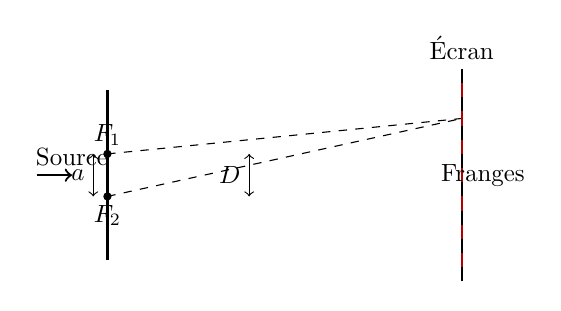
\begin{tikzpicture}[scale=0.9, transform shape]
  % Source et fentes
  \draw[thick,->] (-3,0) -- (-2.5,0) node[above] {Source};
  \draw[thick] (-2,-1.2) -- (-2,1.2);
  \draw[fill=black] (-2,0.3) circle (0.05) node[above] {$F_1$};
  \draw[fill=black] (-2,-0.3) circle (0.05) node[below] {$F_2$};
  \draw[<->] (-2.2,0.3) -- (-2.2,-0.3) node[midway,left] {$a$};
  % Écran
  \draw[thick] (3,-1.5) -- (3,1.5) node[above] {Écran};
  % Rayons
  \draw[dashed] (-2,0.3) -- (3,0.8);
  \draw[dashed] (-2,-0.3) -- (3,0.8);
  \draw[<->] (0,0.3) -- (0,-0.3) node[midway,left] {$D$};
  % Franges (symboliques)
  \foreach \y in {-1.2,-0.8,-0.4,0,0.4,0.8,1.2}
    \draw[thick,red!70!black] (3,\y-0.1) -- (3,\y+0.1);
  \node at (3.3,0) {Franges};
\end{tikzpicture}
\fig{Schéma du dispositif des fentes de Young.}
\end{illus}

\begin{loi}[Condition d'interférence constructive]
Deux ondes issues de \(F_1\) et \(F_2\) interfèrent constructivement (franges brillantes) si leur différence de marche \(\delta\) est un multiple entier de la longueur d'onde :
\[
\delta = k \lambda \quad (k \in \mathbb{Z})
\]
Pour une frange sombre (destructive) :
\[
\delta = (k + \tfrac12) \lambda
\]
\end{loi}

\begin{propriete}[Interfrange]
Dans l'expérience de Young, la distance entre deux franges brillantes consécutives (ou deux franges sombres consécutives) est appelée interfrange \(i\). Elle vaut :
\[
i = \frac{\lambda D}{a}
\]
où \(D\) est la distance fentes-écran et \(a\) la distance entre les deux fentes.
\end{propriete}

\begin{exemple}
Pour une lumière de longueur d'onde \(\lambda = \SI{500}{\nano\metre}\), des fentes distantes de \(a = \SI{0.50}{\milli\metre}\) et un écran à \(D = \SI{2.0}{\metre}\), l'interfrange est :
\[
i = \frac{\SI{500e-9}{\metre} \times \SI{2.0}{\metre}}{\SI{0.50e-3}{\metre}} = \SI{2.0e-3}{\metre} = \SI{2.0}{\milli\metre}
\]
\end{exemple}

\subsection{Diffraction de la lumière}

\begin{definition}[Diffraction]
La diffraction est le phénomène par lequel une onde lumineuse contourne un obstacle ou s'étale après avoir traversé une ouverture de petite dimension (fente, trou). Elle est caractéristique du comportement ondulatoire.
\end{definition}

\begin{experience}[Diffraction par une fente fine]
Un faisceau laser traverse une fente de largeur \(b\) (de l'ordre du dixième de millimètre). Sur un écran, on observe une tache centrale brillante, large, encadrée de taches secondaires moins lumineuses. La largeur angulaire \(\theta\) de la tache centrale vérifie :
\[
\theta \approx \frac{\lambda}{b}
\]
\end{experience}

\begin{illus}
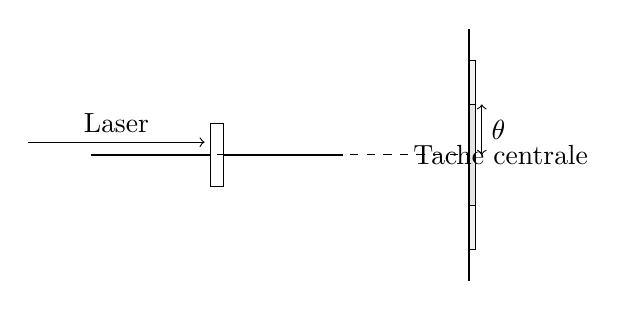
\begin{tikzpicture}[scale=0.8]
  \draw[thick] (-2,0) -- (2,0);
  \draw[thick] (0,-0.5) -- (0,0.5);
  \draw[fill=white] (-0.1,-0.5) rectangle (0.1,0.5);
  \draw[->] (-3,0.2) -- (-0.2,0.2) node[midway,above] {Laser};
  \draw[dashed] (0,0) -- (4,0);
  \draw[thick] (4,-2) -- (4,2);
  \draw[fill=gray!20] (4,-0.8) rectangle (4.1,0.8);
  \draw[fill=gray!10] (4,-1.5) rectangle (4.1,-0.8);
  \draw[fill=gray!10] (4,0.8) rectangle (4.1,1.5);
  \draw[<->] (4.2,0) -- (4.2,0.8) node[midway,right] {$\theta$};
  \node at (4.5,0) {Tache centrale};
\end{tikzpicture}
\fig{Diffraction par une fente fine : tache centrale et taches secondaires.}
\end{illus}

\begin{aretenir}
Les phénomènes d'interférences et de diffraction sont la preuve du caractère ondulatoire de la lumière. Ils ne peuvent s'expliquer par un modèle purement corpusculaire.
\end{aretenir}

% ===================================================================
\section{Aspect corpusculaire : l'effet photoélectrique}

\begin{experience}[Effet photoélectrique]
Lorsqu'une lumière de fréquence suffisamment élevée éclaire une plaque métallique (par exemple du césium ou du zinc), des électrons sont arrachés de la surface. Ce phénomène est appelé effet photoélectrique.
\end{experience}

\begin{remarque}
La théorie ondulatoire classique prévoit que l'énergie des électrons émis devrait augmenter avec l'intensité lumineuse, et que tout éclairement, même de faible fréquence, finirait par arracher des électrons. Or l'expérience montre le contraire : il existe une fréquence seuil en dessous de laquelle aucun électron n'est émis, quelle que soit l'intensité.
\end{remarque}

\begin{loi}[Einstein — 1905]
Pour expliquer l'effet photoélectrique, Einstein propose que la lumière est constituée de grains d'énergie appelés \textbf{photons}. Chaque photon transporte une énergie :
\[
E_{\text{photon}} = h f
\]
où \(h = \SI{6.63e-34}{\joule\second}\) est la constante de Planck.
Lorsqu'un photon frappe la surface métallique, son énergie est transférée à un électron. Une partie de cette énergie sert à extraire l'électron du métal (travail d'extraction \(W_0\)), le reste devient énergie cinétique de l'électron émis :
\[
h f = W_0 + E_c
\]
\end{loi}

\begin{definition}[Travail d'extraction et fréquence seuil]
Le travail d'extraction \(W_0\) est l'énergie minimale nécessaire pour arracher un électron du métal. La fréquence seuil \(f_0\) est la fréquence minimale pour laquelle l'effet photoélectrique se produit :
\[
W_0 = h f_0
\]
Pour \(f < f_0\), aucun électron n'est émis.
\end{definition}

\begin{exemple}
Le césium a un travail d'extraction \(W_0 = \SI{2.14}{\electronvolt}\). Calculons sa fréquence seuil.
\[
W_0 = \SI{2.14}{\electronvolt} = \SI{2.14}{\electronvolt} \times \SI{1.60e-19}{\joule\per\electronvolt} = \SI{3.42e-19}{\joule}
\]
\[
f_0 = \frac{W_0}{h} = \frac{\SI{3.42e-19}{\joule}}{\SI{6.63e-34}{\joule\second}} = \SI{5.16e14}{\hertz}
\]
Cette fréquence correspond à une longueur d'onde \(\lambda_0 = c/f_0 = \SI{581}{\nano\metre}\) (lumière jaune-verte).
\end{exemple}

\begin{aretenir}
L'effet photoélectrique démontre le caractère corpusculaire de la lumière : l'énergie est échangée par paquets discrets (photons). La lumière possède donc une \textbf{dualité onde-particule} : elle se manifeste comme onde dans les interférences et la diffraction, et comme particule dans l'effet photoélectrique.
\end{aretenir}

% ===================================================================
\section{Spectres atomiques et niveaux d'énergie}

\subsection{Spectres d'émission et d'absorption}

\begin{definition}[Spectre de raies]
Un gaz porté à haute température émet une lumière dont le spectre, observé à l'aide d'un spectroscope, est constitué de raies fines et colorées sur fond noir : c'est un \textbf{spectre de raies d'émission}. Chaque élément chimique possède un spectre de raies caractéristique.
\end{definition}

\begin{definition}[Spectre d'absorption]
Lorsqu'une lumière blanche traverse un gaz froid, certaines longueurs d'onde sont absorbées : on observe un spectre continu traversé de raies noires : c'est un \textbf{spectre de raies d'absorption}. Les raies d'absorption d'un élément coïncident exactement avec ses raies d'émission.
\end{definition}

\subsection{Niveaux d'énergie de l'atome}

\begin{loi}[Niveaux d'énergie quantifiés]
L'énergie d'un atome ne peut prendre que certaines valeurs discrètes appelées \textbf{niveaux d'énergie}. Le niveau le plus bas est l'état fondamental (\(E_1\)). Les niveaux supérieurs sont les états excités (\(E_2, E_3, \dots\)).
\end{loi}

\begin{loi}[Transitions électroniques — Bohr]
Un atome peut passer d'un niveau d'énergie \(E_i\) à un niveau supérieur \(E_f\) en absorbant un photon d'énergie :
\[
h f = E_f - E_i
\]
Inversement, lors d'une désexcitation (passage d'un niveau supérieur à un niveau inférieur), l'atome émet un photon d'énergie :
\[
h f = E_i - E_f
\]
\end{loi}

\begin{illus}
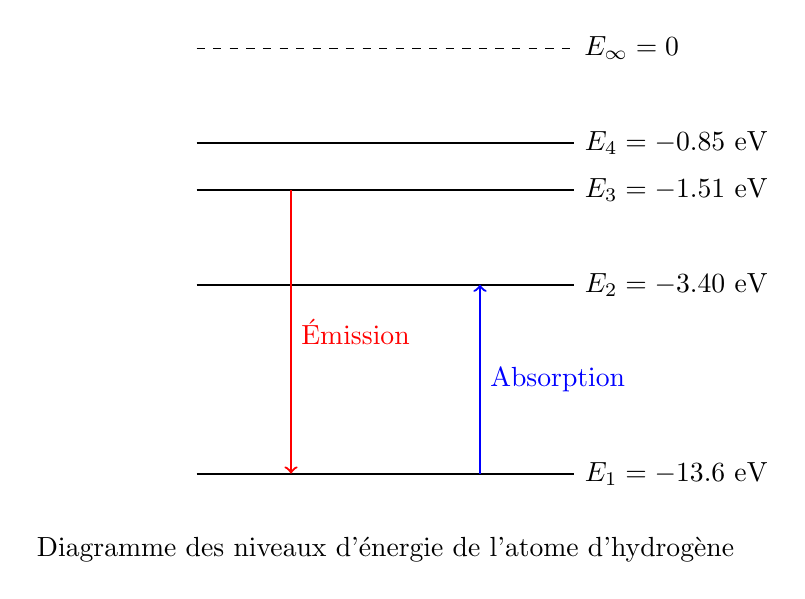
\begin{tikzpicture}[scale=1.2]
  % Niveaux d'énergie
  \draw[thick] (0,0) -- (4,0) node[right] {$E_1 = -13.6\ \mathrm{eV}$};
  \draw[thick] (0,2) -- (4,2) node[right] {$E_2 = -3.40\ \mathrm{eV}$};
  \draw[thick] (0,3) -- (4,3) node[right] {$E_3 = -1.51\ \mathrm{eV}$};
  \draw[thick] (0,3.5) -- (4,3.5) node[right] {$E_4 = -0.85\ \mathrm{eV}$};
  \draw[dashed] (0,4.5) -- (4,4.5) node[right] {$E_\infty = 0$};
  % Flèches d'émission
  \draw[->,red,thick] (1,3) -- (1,0) node[midway,right] {Émission};
  \draw[->,blue,thick] (3,0) -- (3,2) node[midway,right] {Absorption};
  \node at (2,-0.8) {Diagramme des niveaux d'énergie de l'atome d'hydrogène};
\end{tikzpicture}
\fig{Diagramme des niveaux d'énergie de l'atome d'hydrogène (échelle non linéaire).}
\end{illus}

\begin{exemple}
Pour l'atome d'hydrogène, la transition du niveau \(n=3\) (\(E_3 = \SI{-1.51}{\electronvolt}\)) au niveau \(n=2\) (\(E_2 = \SI{-3.40}{\electronvolt}\)) émet un photon d'énergie :
\[
\Delta E = E_3 - E_2 = \SI{1.89}{\electronvolt} = \SI{3.02e-19}{\joule}
\]
La fréquence correspondante est :
\[
f = \frac{\Delta E}{h} = \frac{\SI{3.02e-19}{\joule}}{\SI{6.63e-34}{\joule\second}} = \SI{4.56e14}{\hertz}
\]
et la longueur d'onde \(\lambda = c/f = \SI{658}{\nano\metre}\) (raie rouge de l'hydrogène).
\end{exemple}

\begin{aretenir}
Les spectres de raies sont la signature des niveaux d'énergie quantifiés des atomes. Chaque raie correspond à une transition entre deux niveaux. L'étude des spectres permet d'identifier les éléments chimiques présents dans une source lumineuse (analyse spectrale).
\end{aretenir}

% ===================================================================
\section{L'essentiel à retenir}

\begin{synthese}
\paragraph{Modèle ondulatoire}
\begin{itemize}
  \item La lumière est une onde électromagnétique : \(c = \lambda f\).
  \item \textbf{Interférences} (Young) : franges brillantes si \(\delta = k\lambda\), sombres si \(\delta = (k+1/2)\lambda\). Interfrange : \(i = \lambda D / a\).
  \item \textbf{Diffraction} par une fente : largeur angulaire \(\theta \approx \lambda / b\).
\end{itemize}

\paragraph{Aspect corpusculaire}
\begin{itemize}
  \item Photon : \(E = h f\) avec \(h = \SI{6.63e-34}{\joule\second}\).
  \item Effet photoélectrique : \(h f = W_0 + E_c\). Fréquence seuil : \(f_0 = W_0 / h\).
  \item Dualité onde-particule : la lumière se comporte comme une onde ou comme un flux de photons selon l'expérience.
\end{itemize}

\paragraph{Spectres atomiques}
\begin{itemize}
  \item Niveaux d'énergie quantifiés : \(E_1 < E_2 < E_3 < \dots\).
  \item Transition : \(h f = |E_f - E_i|\).
  \item Spectre de raies d'émission/absorption : signature de chaque élément.
\end{itemize}

\paragraph{Unités importantes}
\begin{itemize}
  \item Longueur d'onde : \si{\metre}, \si{\nano\metre} (\SI{1}{\nano\metre} = \SI{1e-9}{\metre}).
  \item Fréquence : \si{\hertz}.
  \item Énergie : \si{\joule} ou \si{\electronvolt} (\SI{1}{\electronvolt} = \SI{1.60e-19}{\joule}).
  \item Constante de Planck : \(h = \SI{6.63e-34}{\joule\second}\).
\end{itemize}

\paragraph{Plan de résolution pour l'effet photoélectrique}
\begin{enumerate}
  \item Identifier le travail d'extraction \(W_0\) (donné ou à calculer via \(f_0\)).
  \item Calculer l'énergie du photon : \(E = h f\).
  \item Appliquer la conservation de l'énergie : \(E_c = h f - W_0\).
  \item Si \(f < f_0\), pas d'émission.
\end{enumerate}

\paragraph{Attention aux pièges}
\begin{itemize}
  \item Ne pas confondre interfrange \(i\) et distance entre fentes \(a\).
  \item L'énergie cinétique des photoélectrons ne dépend pas de l'intensité lumineuse, mais seulement de la fréquence.
  \item Les niveaux d'énergie sont négatifs (état lié) ; l'énergie d'ionisation est \(|E_1|\).
\end{itemize}
\end{synthese}

% ===================================================================
\section{Méthodes \& savoir-faire}

\methode{Calculer l'interfrange dans l'expérience de Young}
Pour déterminer l'interfrange \(i\), on utilise la formule \(i = \lambda D / a\). Attention aux unités : exprimer toutes les longueurs en mètres. Si on mesure la distance entre \(N\) franges, on a \(i = d / (N-1)\).

\begin{exemple}
Sur un écran placé à \(D = \SI{2.50}{\metre}\) des fentes de Young distantes de \(a = \SI{0.40}{\milli\metre}\), on mesure une distance de \SI{18.0}{\milli\metre} entre 10 franges brillantes. Calculer \(\lambda\).
\[
i = \frac{\SI{18.0e-3}{\metre}}{9} = \SI{2.00e-3}{\metre}
\]
\[
\lambda = \frac{i a}{D} = \frac{\SI{2.00e-3}{\metre} \times \SI{0.40e-3}{\metre}}{\SI{2.50}{\metre}} = \SI{3.20e-7}{\metre} = \SI{320}{\nano\metre}
\]
\end{exemple}

\methode{Exploiter l'effet photoélectrique}
On utilise l'équation d'Einstein : \(h f = W_0 + E_c\). Si on connaît la fréquence seuil, on calcule \(W_0 = h f_0\). L'énergie cinétique maximale des électrons est \(E_{c,\max} = e U_0\) où \(U_0\) est le potentiel d'arrêt.

\begin{exemple}
Une lumière de fréquence \(f = \SI{1.2e15}{\hertz}\) éclaire une cathode de sodium (\(W_0 = \SI{2.28}{\electronvolt}\)). Calculer l'énergie cinétique maximale des électrons émis.
\[
E_{\text{photon}} = h f = \SI{6.63e-34}{\joule\second} \times \SI{1.2e15}{\hertz} = \SI{7.96e-19}{\joule}
\]
\[
W_0 = \SI{2.28}{\electronvolt} = \SI{2.28}{\electronvolt} \times \SI{1.60e-19}{\joule\per\electronvolt} = \SI{3.65e-19}{\joule}
\]
\[
E_c = \SI{7.96e-19}{\joule} - \SI{3.65e-19}{\joule} = \SI{4.31e-19}{\joule} = \SI{2.69}{\electronvolt}
\]
\end{exemple}

\methode{Analyser un spectre de raies}
Chaque raie correspond à une transition entre deux niveaux d'énergie. On calcule l'énergie du photon émis ou absorbé par \(\Delta E = h c / \lambda\). On identifie ensuite les niveaux concernés.

\begin{exemple}
Une raie d'émission de l'hydrogène a pour longueur d'onde \(\lambda = \SI{486}{\nano\metre}\). Calculer l'énergie du photon correspondant.
\[
E = \frac{h c}{\lambda} = \frac{\SI{6.63e-34}{\joule\second} \times \SI{3.00e8}{\metre\per\second}}{\SI{486e-9}{\metre}} = \SI{4.09e-19}{\joule} = \SI{2.56}{\electronvolt}
\]
Cette raie correspond à la transition \(n=4 \to n=2\) (série de Balmer).
\end{exemple}

\methode{Utiliser la dualité onde-particule}
Pour un photon, la longueur d'onde \(\lambda\) et la quantité de mouvement \(p\) sont liées par \(p = h / \lambda\). Cette relation est utilisée en mécanique quantique pour décrire le comportement des particules matérielles (onde de matière).

\begin{exemple}
Un photon de longueur d'onde \(\lambda = \SI{500}{\nano\metre}\) a une quantité de mouvement :
\[
p = \frac{h}{\lambda} = \frac{\SI{6.63e-34}{\joule\second}}{\SI{500e-9}{\metre}} = \SI{1.33e-27}{\kilogram\metre\per\second}
\]
\end{exemple}

\methode{Calculer l'énergie d'ionisation}
L'énergie d'ionisation est l'énergie nécessaire pour arracher un électron de l'état fondamental. Elle vaut \(E_{\text{ion}} = |E_1|\). Pour l'hydrogène, \(E_1 = \SI{-13.6}{\electronvolt}\), donc \(E_{\text{ion}} = \SI{13.6}{\electronvolt}\).

\begin{exemple}
Quelle est la longueur d'onde maximale d'un photon capable d'ioniser un atome d'hydrogène dans son état fondamental ?
\[
\lambda_{\max} = \frac{h c}{E_{\text{ion}}} = \frac{\SI{6.63e-34}{\joule\second} \times \SI{3.00e8}{\metre\per\second}}{\SI{13.6}{\electronvolt} \times \SI{1.60e-19}{\joule\per\electronvolt}} = \SI{9.13e-8}{\metre} = \SI{91.3}{\nano\metre}
\]
Cette longueur d'onde se situe dans l'ultraviolet.
\end{exemple}

\methode{Interpréter un diagramme de niveaux d'énergie}
Sur un diagramme, les transitions possibles sont représentées par des flèches verticales. La longueur de la flèche est proportionnelle à l'énergie du photon émis ou absorbé. Plus la transition est grande, plus la fréquence est élevée et plus la longueur d'onde est courte.

\begin{exemple}
Sur le diagramme de l'hydrogène, la transition \(n=2 \to n=1\) émet un photon d'énergie \(\Delta E = \SI{10.2}{\electronvolt}\) (ultraviolet), tandis que \(n=3 \to n=2\) émet \(\Delta E = \SI{1.89}{\electronvolt}\) (rouge visible).
\end{exemple}

\methode{Distinguer spectre d'émission et d'absorption}
Un spectre d'émission présente des raies brillantes sur fond noir (gaz chaud). Un spectre d'absorption présente des raies noires sur fond continu (lumière blanche traversant un gaz froid). Les positions des raies coïncident pour un même élément.

\begin{exemple}
Le spectre du sodium présente une double raie jaune à \(\lambda = \SI{589.0}{\nano\metre}\) et \(\SI{589.6}{\nano\metre}\). Ces mêmes raies apparaissent en absorption dans le spectre solaire (raies de Fraunhofer).
\end{exemple}

\methode{Appliquer la conservation de l'énergie dans une transition}
Lors d'une transition, l'énergie totale est conservée : l'énergie perdue par l'atome est exactement égale à l'énergie du photon émis (ou gagnée pour un photon absorbé). On écrit \(h f = |E_f - E_i|\).

\begin{exemple}
Un atome d'hydrogène passe de \(n=4\) (\(E_4 = \SI{-0.85}{\electronvolt}\)) à \(n=2\) (\(E_2 = \SI{-3.40}{\electronvolt}\)). L'énergie du photon émis est :
\[
\Delta E = \SI{3.40}{\electronvolt} - \SI{0.85}{\electronvolt} = \SI{2.55}{\electronvolt}
\]
La fréquence est \(f = \Delta E / h = \SI{6.15e14}{\hertz}\) et la longueur d'onde \(\lambda = \SI{488}{\nano\metre}\) (bleu-vert).
\end{exemple}

% ===================================================================
\section{Exercices d'application}

\rubrique{Interférences lumineuses}

\exo{}\diff{1}
Dans l'expérience de Young, on utilise une lumière de longueur d'onde \(\lambda = \SI{550}{\nano\metre}\). La distance entre les fentes est \(a = \SI{0.30}{\milli\metre}\) et l'écran est à \(D = \SI{1.50}{\metre}\). Calculer l'interfrange \(i\).

\exo{}\diff{2}
On réalise l'expérience de Young avec une lumière monochromatique. On mesure une distance de \SI{12.0}{\milli\metre} entre 8 franges brillantes. La distance fentes-écran est \(D = \SI{2.00}{\metre}\) et la distance entre les fentes est \(a = \SI{0.50}{\milli\metre}\). Déterminer la longueur d'onde de la lumière utilisée.

\exo{}\diff{2}
Deux fentes de Young sont distantes de \(a = \SI{0.20}{\milli\metre}\). L'écran est à \(D = \SI{1.00}{\metre}\). On observe que la 5e frange brillante (hors frange centrale) est à \SI{15.0}{\milli\metre} du centre. Calculer la longueur d'onde de la lumière.

\rubrique{Diffraction}

\exo{}\diff{1}
Un faisceau laser (\(\lambda = \SI{632.8}{\nano\metre}\)) traverse une fente de largeur \(b = \SI{0.10}{\milli\metre}\). Calculer la largeur angulaire \(\theta\) de la tache centrale de diffraction.

\exo{}\diff{2}
La tache centrale de diffraction d'un laser (\(\lambda = \SI{532}{\nano\metre}\)) a une largeur de \SI{5.0}{\centi\metre} sur un écran situé à \(D = \SI{2.0}{\metre}\). Quelle est la largeur \(b\) de la fente ?

\rubrique{Effet photoélectrique}

\exo{}\diff{1}
Le travail d'extraction du potassium est \(W_0 = \SI{2.25}{\electronvolt}\). Calculer sa fréquence seuil \(f_0\) et sa longueur d'onde seuil \(\lambda_0\).

\exo{}\diff{2}
Une lumière de fréquence \(f = \SI{8.0e14}{\hertz}\) éclaire une cathode de césium (\(W_0 = \SI{2.14}{\electronvolt}\)). Les électrons émis sont arrêtés par un potentiel \(U_0\). Calculer \(U_0\).

\exo{}\diff{3}
On éclaire une plaque de sodium (\(W_0 = \SI{2.28}{\electronvolt}\)) avec une lumière de longueur d'onde \(\lambda = \SI{400}{\nano\metre}\). Déterminer :
\begin{enumerate}
  \item L'énergie du photon incident.
  \item L'énergie cinétique maximale des électrons émis.
  \item La vitesse maximale des électrons (masse de l'électron \(m_e = \SI{9.11e-31}{\kilogram}\)).
\end{enumerate}

\rubrique{Spectres et niveaux d'énergie}

\exo{}\diff{1}
L'atome d'hydrogène possède les niveaux d'énergie suivants : \(E_1 = \SI{-13.6}{\electronvolt}\), \(E_2 = \SI{-3.40}{\electronvolt}\), \(E_3 = \SI{-1.51}{\electronvolt}\), \(E_4 = \SI{-0.85}{\electronvolt}\). Calculer l'énergie du photon émis lors de la transition \(n=4 \to n=2\).

\exo{}\diff{2}
Une raie d'émission de l'hydrogène a pour longueur d'onde \(\lambda = \SI{656}{\nano\metre}\). À quelle transition correspond-elle ?

\exo{}\diff{2}
Un atome d'hydrogène dans son état fondamental absorbe un photon de longueur d'onde \(\lambda = \SI{97.2}{\nano\metre}\). À quel niveau l'électron est-il excité ?

\rubrique{Dualité onde-particule}

\exo{}\diff{2}
Calculer la quantité de mouvement d'un photon de longueur d'onde \(\lambda = \SI{500}{\nano\metre}\). En déduire sa masse équivalente (utiliser \(E = m c^2\)).

\exo{}\diff{3}
Un électron est accéléré par une tension \(U = \SI{100}{\volt}\). Sa longueur d'onde de de Broglie est \(\lambda = h / p\). Calculer \(\lambda\) (masse de l'électron \(m_e = \SI{9.11e-31}{\kilogram}\), charge \(e = \SI{1.60e-19}{\coulomb}\)).

% ===================================================================
\section{Exercices d'entraînement}

\rubrique{Interférences et diffraction}

\exo{}\diff{2}
Dans un dispositif de Young, on utilise une lumière de longueur d'onde \(\lambda = \SI{589}{\nano\metre}\). La distance entre les fentes est \(a = \SI{0.25}{\milli\metre}\) et l'écran est à \(D = \SI{1.20}{\metre}\). Calculer la distance entre la frange centrale et la 3e frange brillante.

\exo{}\diff{2}
On remplace la lumière précédente par une lumière de longueur d'onde inconnue. La distance entre la frange centrale et la 4e frange brillante est de \SI{14.4}{\milli\metre}. Déterminer \(\lambda\).

\exo{}\diff{3}
Deux fentes de Young sont distantes de \(a = \SI{0.15}{\milli\metre}\). L'écran est à \(D = \SI{0.80}{\metre}\). On observe que la 6e frange sombre (hors frange centrale) est à \SI{16.0}{\milli\metre} du centre. Calculer la longueur d'onde.

\exo{}\diff{2}
Un faisceau laser (\(\lambda = \SI{632.8}{\nano\metre}\)) éclaire une fente de largeur \(b = \SI{0.08}{\milli\metre}\). Sur un écran à \(D = \SI{1.50}{\metre}\), quelle est la largeur de la tache centrale de diffraction ?

\exo{}\diff{3}
La tache centrale de diffraction d'un laser (\(\lambda = \SI{532}{\nano\metre}\)) a une largeur de \SI{8.0}{\centi\metre} sur un écran à \(D = \SI{2.5}{\metre}\). Quelle est la largeur de la fente ?

\rubrique{Effet photoélectrique}

\exo{}\diff{2}
Le travail d'extraction du tungstène est \(W_0 = \SI{4.52}{\electronvolt}\). Quelle est la fréquence seuil ? Quelle est la longueur d'onde seuil ?

\exo{}\diff{2}
Une lumière de longueur d'onde \(\lambda = \SI{300}{\nano\metre}\) éclaire une cathode de césium (\(W_0 = \SI{2.14}{\electronvolt}\)). Calculer l'énergie cinétique maximale des électrons émis.

\exo{}\diff{3}
On éclaire une plaque de sodium (\(W_0 = \SI{2.28}{\electronvolt}\)) avec une lumière de fréquence \(f = \SI{1.0e15}{\hertz}\). Calculer le potentiel d'arrêt \(U_0\).

\exo{}\diff{3}
Une cellule photoélectrique au césium (\(W_0 = \SI{2.14}{\electronvolt}\)) est éclairée par une lumière de puissance \(P = \SI{1.0}{\milli\watt}\) et de longueur d'onde \(\lambda = \SI{500}{\nano\metre}\). Calculer le nombre de photons émis par seconde, puis le nombre d'électrons émis par seconde (rendement quantique = 1).

\rubrique{Spectres et niveaux d'énergie}

\exo{}\diff{2}
L'atome d'hydrogène a les niveaux d'énergie suivants : \(E_1 = \SI{-13.6}{\electronvolt}\), \(E_2 = \SI{-3.40}{\electronvolt}\), \(E_3 = \SI{-1.51}{\electronvolt}\), \(E_4 = \SI{-0.85}{\electronvolt}\). Calculer les longueurs d'onde des transitions \(n=3 \to n=1\), \(n=4 \to n=1\) et \(n=5 \to n=2\) (on donne \(E_5 = \SI{-0.54}{\electronvolt}\)).

\exo{}\diff{3}
Un atome d'hydrogène dans son état fondamental absorbe un photon de longueur d'onde \(\lambda = \SI{102.6}{\nano\metre}\). À quel niveau l'électron est-il excité ? Quelle est l'énergie d'ionisation de l'hydrogène ?

\exo{}\diff{2}
Le spectre d'émission de l'hydrogène présente une raie à \(\lambda = \SI{434}{\nano\metre}\). À quelle transition correspond-elle ?

\rubrique{Dualité onde-particule}

\exo{}\diff{2}
Calculer la longueur d'onde de de Broglie d'un électron de vitesse \(v = \SI{2.0e6}{\metre\per\second}\) (masse \(m_e = \SI{9.11e-31}{\kilogram}\)).

\exo{}\diff{3}
Un neutron thermique a une énergie cinétique \(E_c = \SI{0.025}{\electronvolt}\). Calculer sa longueur d'onde de de Broglie (masse du neutron \(m_n = \SI{1.67e-27}{\kilogram}\)).

\exo{}\diff{3}
Un faisceau d'électrons accélérés par une tension \(U\) produit une figure de diffraction sur un cristal. La première tache de diffraction apparaît pour un angle \(\theta = \ang{30}\). Sachant que la distance interréticulaire du cristal est \(d = \SI{0.20}{\nano\metre}\), calculer \(U\) (utiliser la relation de Bragg \(2d \sin\theta = n\lambda\) avec \(n=1\)).

% ===================================================================
\section{Sujets type Baccalauréat}

\sujetbac[Interférences et effet photoélectrique]
\paragraph{Partie A : Interférences lumineuses}
On réalise l'expérience des fentes de Young avec une lumière monochromatique de longueur d'onde \(\lambda = \SI{546}{\nano\metre}\). La distance entre les fentes est \(a = \SI{0.30}{\milli\metre}\) et l'écran est à \(D = \SI{2.00}{\metre}\).

\begin{enumerate}
  \item Calculer l'interfrange \(i\).
  \item On mesure une distance de \SI{21.8}{\milli\metre} entre plusieurs franges brillantes. Combien de franges a-t-on mesurées ?
  \item On remplace la lumière par une autre de longueur d'onde inconnue. L'interfrange devient \(i' = \SI{4.0}{\milli\metre}\). Calculer \(\lambda'\).
\end{enumerate}

\paragraph{Partie B : Effet photoélectrique}
Une cellule photoélectrique au césium (\(W_0 = \SI{2.14}{\electronvolt}\)) est éclairée par une lumière de fréquence \(f = \SI{7.5e14}{\hertz}\).

\begin{enumerate}
  \item Montrer que l'effet photoélectrique se produit.
  \item Calculer l'énergie cinétique maximale des électrons émis.
  \item On applique une tension d'arrêt \(U_0\). Calculer \(U_0\).
  \item Quelle serait l'énergie cinétique maximale si on doublait l'intensité lumineuse ? Justifier.
\end{enumerate}

\sujetbac[Spectre de l'hydrogène et dualité]
\paragraph{Partie A : Niveaux d'énergie de l'hydrogène}
On donne les niveaux d'énergie de l'atome d'hydrogène : \(E_n = -\SI{13.6}{\electronvolt} / n^2\).

\begin{enumerate}
  \item Calculer \(E_1\), \(E_2\), \(E_3\) et \(E_4\).
  \item Un atome passe de \(n=4\) à \(n=2\). Calculer l'énergie du photon émis.
  \item En déduire la fréquence et la longueur d'onde de la raie correspondante.
  \item À quelle série de raies appartient cette transition ?
\end{enumerate}

\paragraph{Partie B : Dualité onde-particule}
Un faisceau d'électrons est accéléré par une tension \(U = \SI{150}{\volt}\).

\begin{enumerate}
  \item Calculer la vitesse des électrons.
  \item Calculer leur longueur d'onde de de Broglie.
  \item Ce faisceau est utilisé pour une expérience de diffraction par un cristal. Expliquer pourquoi on observe une figure de diffraction.
\end{enumerate}

\sujetbac[Diffraction et analyse spectrale]
\paragraph{Partie A : Diffraction}
Un laser de longueur d'onde \(\lambda = \SI{632.8}{\nano\metre}\) éclaire une fente de largeur \(b = \SI{0.12}{\milli\metre}\). Sur un écran à \(D = \SI{1.80}{\metre}\), on observe une figure de diffraction.

\begin{enumerate}
  \item Calculer la largeur angulaire \(\theta\) de la tache centrale.
  \item En déduire la largeur de la tache centrale sur l'écran.
  \item Que devient cette largeur si on double la largeur de la fente ?
\end{enumerate}

\paragraph{Partie B : Analyse spectrale}
On analyse la lumière émise par une lampe à vapeur de sodium à l'aide d'un spectroscope. On observe deux raies jaunes très proches : \(\lambda_1 = \SI{589.0}{\nano\metre}\) et \(\lambda_2 = \SI{589.6}{\nano\metre}\).

\begin{enumerate}
  \item Calculer les fréquences correspondantes.
  \item Calculer l'énergie des photons pour chaque raie.
  \item Expliquer pourquoi ces deux raies sont caractéristiques du sodium.
  \item Comment pourrait-on vérifier que ces raies correspondent à des transitions entre niveaux d'énergie ?
\end{enumerate}

% ===================================================================
\section{Corrigés}

\corrige{de l'exercice 1}
\[
i = \frac{\lambda D}{a} = \frac{\SI{550e-9}{\metre} \times \SI{1.50}{\metre}}{\SI{0.30e-3}{\metre}} = \SI{2.75e-3}{\metre} = \SI{2.75}{\milli\metre}
\]

\corrige{de l'exercice 2}
Distance entre 8 franges brillantes = 7 interfranges.
\[
i = \frac{\SI{12.0e-3}{\metre}}{7} = \SI{1.71e-3}{\metre}
\]
\[
\lambda = \frac{i a}{D} = \frac{\SI{1.71e-3}{\metre} \times \SI{0.50e-3}{\metre}}{\SI{2.00}{\metre}} = \SI{4.28e-7}{\metre} = \SI{428}{\nano\metre}
\]

\corrige{de l'exercice 3}
La 5e frange brillante correspond à \(k=5\) (frange centrale \(k=0\)).
\[
\delta = k \lambda = \frac{a x}{D} \quad \Rightarrow \quad \lambda = \frac{a x}{k D} = \frac{\SI{0.20e-3}{\metre} \times \SI{15.0e-3}{\metre}}{5 \times \SI{1.00}{\metre}} = \SI{6.00e-7}{\metre} = \SI{600}{\nano\metre}
\]

\corrige{de l'exercice 4}
\[
\theta \approx \frac{\lambda}{b} = \frac{\SI{632.8e-9}{\metre}}{\SI{0.10e-3}{\metre}} = \SI{6.33e-3}{\radian}
\]

\corrige{de l'exercice 5}
Largeur de la tache centrale = \(2 \theta D\).
\[
\theta = \frac{\text{largeur}}{2 D} = \frac{\SI{5.0e-2}{\metre}}{2 \times \SI{2.0}{\metre}} = \SI{1.25e-2}{\radian}
\]
\[
b = \frac{\lambda}{\theta} = \frac{\SI{532e-9}{\metre}}{\SI{1.25e-2}{\radian}} = \SI{4.26e-5}{\metre} = \SI{42.6}{\micro\metre}
\]

\corrige{de l'exercice 6}
\[
W_0 = \SI{2.25}{\electronvolt} = \SI{2.25}{\electronvolt} \times \SI{1.60e-19}{\joule\per\electronvolt} = \SI{3.60e-19}{\joule}
\]
\[
f_0 = \frac{W_0}{h} = \frac{\SI{3.60e-19}{\joule}}{\SI{6.63e-34}{\joule\second}} = \SI{5.43e14}{\hertz}
\]
\[
\lambda_0 = \frac{c}{f_0} = \frac{\SI{3.00e8}{\metre\per\second}}{\SI{5.43e14}{\hertz}} = \SI{5.52e-7}{\metre} = \SI{552}{\nano\metre}
\]

\corrige{de l'exercice 7}
Énergie du photon :
\[
E = h f = \SI{6.63e-34}{\joule\second} \times \SI{8.0e14}{\hertz} = \SI{5.30e-19}{\joule}
\]
\[
W_0 = \SI{2.14}{\electronvolt} = \SI{3.42e-19}{\joule}
\]
\[
E_c = E - W_0 = \SI{5.30e-19}{\joule} - \SI{3.42e-19}{\joule} = \SI{1.88e-19}{\joule}
\]
\[
U_0 = \frac{E_c}{e} = \frac{\SI{1.88e-19}{\joule}}{\SI{1.60e-19}{\coulomb}} = \SI{1.18}{\volt}
\]

\corrige{de l'exercice 8}
\begin{enumerate}
  \item \(E = \frac{h c}{\lambda} = \frac{\SI{6.63e-34}{\joule\second} \times \SI{3.00e8}{\metre\per\second}}{\SI{400e-9}{\metre}} = \SI{4.97e-19}{\joule} = \SI{3.11}{\electronvolt}\)
  \item \(E_c = E - W_0 = \SI{3.11}{\electronvolt} - \SI{2.28}{\electronvolt} = \SI{0.83}{\electronvolt} = \SI{1.33e-19}{\joule}\)
  \item \(v = \sqrt{\frac{2 E_c}{m_e}} = \sqrt{\frac{2 \times \SI{1.33e-19}{\joule}}{\SI{9.11e-31}{\kilogram}}} = \SI{5.40e5}{\metre\per\second}\)
\end{enumerate}

\corrige{de l'exercice 9}
\[
\Delta E = E_4 - E_2 = \SI{-0.85}{\electronvolt} - (\SI{-3.40}{\electronvolt}) = \SI{2.55}{\electronvolt} = \SI{4.08e-19}{\joule}
\]

\corrige{de l'exercice 10}
\[
E = \frac{h c}{\lambda} = \frac{\SI{6.63e-34}{\joule\second} \times \SI{3.00e8}{\metre\per\second}}{\SI{656e-9}{\metre}} = \SI{3.03e-19}{\joule} = \SI{1.89}{\electronvolt}
\]
Cette énergie correspond à la transition \(n=3 \to n=2\) (car \(E_3 - E_2 = \SI{1.51}{\electronvolt} - (\SI{-3.40}{\electronvolt}) = \SI{1.89}{\electronvolt}\)).

\corrige{de l'exercice 11}
\[
E = \frac{h c}{\lambda} = \frac{\SI{6.63e-34}{\joule\second} \times \SI{3.00e8}{\metre\per\second}}{\SI{97.2e-9}{\metre}} = \SI{2.05e-18}{\joule} = \SI{12.8}{\electronvolt}
\]
L'atome passe de \(E_1 = \SI{-13.6}{\electronvolt}\) à \(E_f = E_1 + E = \SI{-13.6}{\electronvolt} + \SI{12.8}{\electronvolt} = \SI{-0.8}{\electronvolt}\). Le niveau le plus proche est \(n=4\) (\(E_4 = \SI{-0.85}{\electronvolt}\)). L'électron est excité au niveau \(n=4\).

\corrige{de l'exercice 12}
\[
p = \frac{h}{\lambda} = \frac{\SI{6.63e-34}{\joule\second}}{\SI{500e-9}{\metre}} = \SI{1.33e-27}{\kilogram\metre\per\second}
\]
Masse équivalente : \(m = \frac{E}{c^2} = \frac{h f}{c^2} = \frac{h}{\lambda c} = \frac{\SI{6.63e-34}{\joule\second}}{\SI{500e-9}{\metre} \times \SI{3.00e8}{\metre\per\second}} = \SI{4.42e-36}{\kilogram}\)

\corrige{de l'exercice 13}
Énergie cinétique de l'électron : \(E_c = e U = \SI{1.60e-19}{\coulomb} \times \SI{100}{\volt} = \SI{1.60e-17}{\joule}\)
Vitesse : \(v = \sqrt{\frac{2 E_c}{m_e}} = \sqrt{\frac{2 \times \SI{1.60e-17}{\joule}}{\SI{9.11e-31}{\kilogram}}} = \SI{5.93e6}{\metre\per\second}\)
Quantité de mouvement : \(p = m_e v = \SI{9.11e-31}{\kilogram} \times \SI{5.93e6}{\metre\per\second} = \SI{5.40e-24}{\kilogram\metre\per\second}\)
Longueur d'onde : \(\lambda = \frac{h}{p} = \frac{\SI{6.63e-34}{\joule\second}}{\SI{5.40e-24}{\kilogram\metre\per\second}} = \SI{1.23e-10}{\metre} = \SI{0.123}{\nano\metre}\)

\corrige{du sujet 1}
\paragraph{Partie A}
\begin{enumerate}
  \item \(i = \frac{\lambda D}{a} = \frac{\SI{546e-9}{\metre} \times \SI{2.00}{\metre}}{\SI{0.30e-3}{\metre}} = \SI{3.64e-3}{\metre} = \SI{3.64}{\milli\metre}\)
  \item Nombre d'interfranges = \(\frac{\SI{21.8}{\milli\metre}}{\SI{3.64}{\milli\metre}} = 6\). Donc nombre de franges = 7 (car \(N\) franges donnent \(N-1\) interfranges).
  \item \(\lambda' = \frac{i' a}{D} = \frac{\SI{4.0e-3}{\metre} \times \SI{0.30e-3}{\metre}}{\SI{2.00}{\metre}} = \SI{6.0e-7}{\metre} = \SI{600}{\nano\metre}\)
\end{enumerate}

\paragraph{Partie B}
\begin{enumerate}
  \item \(f_0 = \frac{W_0}{h} = \frac{\SI{2.14}{\electronvolt} \times \SI{1.60e-19}{\joule\per\electronvolt}}{\SI{6.63e-34}{\joule\second}} = \SI{5.16e14}{\hertz}\). \(f = \SI{7.5e14}{\hertz} > f_0\), donc effet photoélectrique.
  \item \(E_c = h f - W_0 = \SI{6.63e-34}{\joule\second} \times \SI{7.5e14}{\hertz} - \SI{3.42e-19}{\joule} = \SI{4.97e-19}{\joule} - \SI{3.42e-19}{\joule} = \SI{1.55e-19}{\joule} = \SI{0.969}{\electronvolt}\)
  \item \(U_0 = \frac{E_c}{e} = \frac{\SI{1.55e-19}{\joule}}{\SI{1.60e-19}{\coulomb}} = \SI{0.969}{\volt}\)
  \item L'énergie cinétique maximale ne dépend pas de l'intensité lumineuse, seulement de la fréquence. Donc \(E_c\) reste inchangée.
\end{enumerate}

\corrige{du sujet 2}
\paragraph{Partie A}
\begin{enumerate}
  \item \(E_1 = -\SI{13.6}{\electronvolt}\), \(E_2 = -\SI{3.40}{\electronvolt}\), \(E_3 = -\SI{1.51}{\electronvolt}\), \(E_4 = -\SI{0.85}{\electronvolt}\)
  \item \(\Delta E = E_4 - E_2 = \SI{2.55}{\electronvolt} = \SI{4.08e-19}{\joule}\)
  \item \(f = \frac{\Delta E}{h} = \frac{\SI{4.08e-19}{\joule}}{\SI{6.63e-34}{\joule\second}} = \SI{6.15e14}{\hertz}\) ; \(\lambda = \frac{c}{f} = \frac{\SI{3.00e8}{\metre\per\second}}{\SI{6.15e14}{\hertz}} = \SI{4.88e-7}{\metre} = \SI{488}{\nano\metre}\)
  \item Cette transition appartient à la série de Balmer (transitions vers \(n=2\)).
\end{enumerate}

\paragraph{Partie B}
\begin{enumerate}
  \item \(E_c = e U = \SI{1.60e-19}{\coulomb} \times \SI{150}{\volt} = \SI{2.40e-17}{\joule}\) ; \(v = \sqrt{\frac{2 E_c}{m_e}} = \sqrt{\frac{2 \times \SI{2.40e-17}{\joule}}{\SI{9.11e-31}{\kilogram}}} = \SI{7.26e6}{\metre\per\second}\)
  \item \(p = m_e v = \SI{9.11e-31}{\kilogram} \times \SI{7.26e6}{\metre\per\second} = \SI{6.61e-24}{\kilogram\metre\per\second}\) ; \(\lambda = \frac{h}{p} = \frac{\SI{6.63e-34}{\joule\second}}{\SI{6.61e-24}{\kilogram\metre\per\second}} = \SI{1.00e-10}{\metre} = \SI{0.100}{\nano\metre}\)
  \item La longueur d'onde des électrons est de l'ordre de la distance interatomique dans un cristal, ce qui permet d'observer une figure de diffraction (phénomène ondulatoire).
\end{enumerate}

\corrige{du sujet 3}
\paragraph{Partie A}
\begin{enumerate}
  \item \(\theta \approx \frac{\lambda}{b} = \frac{\SI{632.8e-9}{\metre}}{\SI{0.12e-3}{\metre}} = \SI{5.27e-3}{\radian}\)
  \item Largeur = \(2 \theta D = 2 \times \SI{5.27e-3}{\radian} \times \SI{1.80}{\metre} = \SI{1.90e-2}{\metre} = \SI{1.90}{\centi\metre}\)
  \item Si on double \(b\), \(\theta\) est divisé par 2, donc la largeur est divisée par 2.
\end{enumerate}

\paragraph{Partie B}
\begin{enumerate}
  \item \(f_1 = \frac{c}{\lambda_1} = \frac{\SI{3.00e8}{\metre\per\second}}{\SI{589.0e-9}{\metre}} = \SI{5.093e14}{\hertz}\) ; \(f_2 = \frac{c}{\lambda_2} = \frac{\SI{3.00e8}{\metre\per\second}}{\SI{589.6e-9}{\metre}} = \SI{5.088e14}{\hertz}\)
  \item \(E_1 = h f_1 = \SI{6.63e-34}{\joule\second} \times \SI{5.093e14}{\hertz} = \SI{3.377e-19}{\joule} = \SI{2.111}{\electronvolt}\) ; \(E_2 = h f_2 = \SI{6.63e-34}{\joule\second} \times \SI{5.088e14}{\hertz} = \SI{3.374e-19}{\joule} = \SI{2.109}{\electronvolt}\)
  \item Ces deux raies sont caractéristiques du sodium car elles correspondent à des transitions entre niveaux d'énergie spécifiques de l'atome de sodium.
  \item On pourrait vérifier en mesurant les longueurs d'onde avec un spectroscope de haute résolution et en les comparant aux valeurs tabulées. On pourrait aussi étudier le diagramme des niveaux d'énergie du sodium pour identifier les transitions correspondantes.
\end{enumerate}